\chapter{The Theory of Alignment}
\label{sec:alignTheory}

Whenever a new detector is built, people are careful to mount it as close to the correct location as they can. In order to check this, survey measurements are
performed to check the position with a precision of $\SI{100}{\micro\metre}$.
To achieve an even greater precision, \textit{software alignment} is performed.

The reason why alignment is of great importance is that a misaligned detector
yields worse momentum resolutions, low reconstruction efficiencies and biased mass estimations and mass peak resolutions.
The most prominent area of misalignment for a spectrometer are asymmetries.
In the past, alignment solved problems for example a Muon asymmetry in the
L0Muon trigger in 2011 and a misalignment in IT boxes which resulted in trigger inefficency regarding $J/\Psi$ in 2012.
% references

\section{Clustering of SciFi hits}
\label{sec:clustering}

The signals generated by the SiPMs are read out by a specifically developed integrated circuit, the \textit{PACIFIC}\footnote{(low Power Asic for the sCIntillating Fibres traCker}\cite{readout}.
It performs the shaping, integration and digitization of the signal. An effect called spillover caused by the propagation delay of photons inside the fibres and the recovery time of the SiPMs. This leads to the signal not being completely inside of its 25-ns timeslot for the bunch crossing. The \textit{PACIFIC} shapes the signal from the SiPM to reduce the spillover and suppress the signal tails\cite{techreport}. Afterwards, the signal is integrated over the 25-ns timeslot and a 2-bit analog-digital converter (ADC) digitizes the signal.
Three comparators implement the ADC and can be set individually for each channel, as seen in figure \ref{fig:pac}.

\begin{figure}
    \centering
    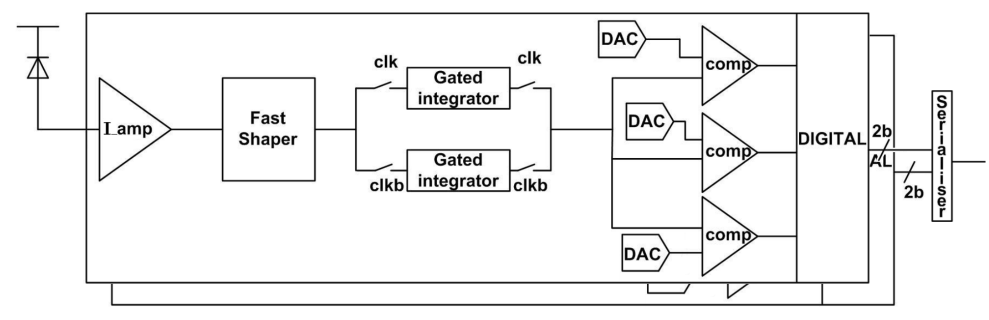
\includegraphics[width=0.8\textwidth]{plots/pacific.png}
    \caption{Figure of the PACIFIC chip. From left to right, an amplifier, a shaper and an integrator are build in. The Signal the is digitized and the Clustering is performed to the 2-bit output on the far right.}
    \label{fig:pac}
\end{figure}

To achieve a reduction in data rate and suppress the signal noise, clusterization is performed. A diagram of the clusterization is shown in Figure \ref{fig:tikz_cluster}

\begin{figure}
  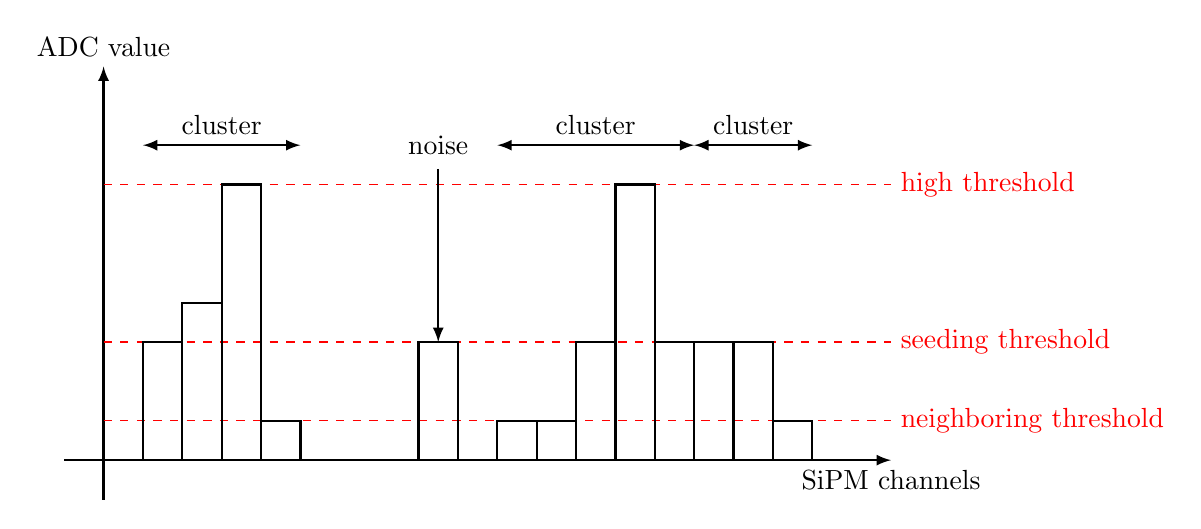
\begin{tikzpicture}
    % coordinates
    \draw[thick, black, -latex] (-0.5, 0) -- (10, 0) node [below] {SiPM channels};
    \draw[thick, black, -latex] (0, -0.5) -- (0, 5) node [above] {ADC value};
    % red lines
    \draw[dashed, red] (0, 0.5) -- (10, 0.5) node [above, right] {neighboring threshold};
    \draw[dashed, red] (0, 1.5) -- (10, 1.5) node [above, right] {seeding threshold};
    \draw[dashed, red] (0, 3.5) -- (10, 3.5) node [above, right] {high threshold};
    % clusters
    \draw[thick, black] (0.5, 0) -- (0.5, 1.5) -- (1, 1.5) -- (1, 0);
    \draw[thick, black] (1, 0) -- (1, 2) -- (1.5, 2) -- (1.5, 0);
    \draw[thick, black] (1.5, 0) -- (1.5, 3.5) -- (2, 3.5) -- (2, 0);
    \draw[thick, black] (2, 0) -- (2, 0.5) -- (2.5, 0.5) -- (2.5, 0);

    \draw[thick, black] (4, 0) -- (4, 1.5) -- (4.5, 1.5) -- (4.5, 0);

    \draw[thick, black] (5, 0) -- (5, 0.5) -- (5.5, 0.5) -- (5.5, 0);
    \draw[thick, black] (11/2, 0) -- (11/2, 1/2) -- (12/2, 1/2) -- (12/2, 0);
    \draw[thick, black] (12/2, 0) -- (12/2, 3/2) -- (13/2, 3/2) -- (13/2, 0);
    \draw[thick, black] (13/2, 0) -- (13/2, 7/2) -- (14/2, 7/2) -- (14/2, 0);
    \draw[thick, black] (14/2, 0) -- (14/2, 3/2) -- (15/2, 3/2) -- (15/2, 0);
    \draw[thick, black] (15/2, 0) -- (15/2, 3/2) -- (16/2, 3/2) -- (16/2, 0);
    \draw[thick, black] (16/2, 0) -- (16/2, 3/2) -- (17/2, 3/2) -- (17/2, 0);
    \draw[thick, black] (17/2, 0) -- (17/2, 1/2) -- (18/2, 1/2) -- (18/2, 0);

    % draw node cluster 1
    \draw[thick, black, latex-latex] (0.5, 4) -- (2.5, 4) node [above, midway] {cluster};

    % draw node cluster 2
    \draw[thick, black, -latex] (8.5/2, 3.7) -- (8.5/2, 1.5);
    \draw (8.5/2, 4) node {noise};

    % draw node cluster 3.1
    \draw[thick, black, latex-latex] (5, 4) -- (7.5, 4) node [above, midway] {cluster};

    % draw node cluster 3.1
    \draw[thick, black, latex-latex] (7.5, 4) -- (9, 4) node [above, midway] {cluster};
  \end{tikzpicture}
  \caption{Clusters are created by a group of channels from which one must be above the seeding threshold and the other channels being above the neighboring threshold. The other option is for one cluster being above the high threshold. Cluster with a width larger than four channels.}
  \label{fig:tikz_cluster}
\end{figure}


During the digitization the specific thresholds are set. The second comparator sets the \textit{seeding threshold} which marks channels exceeding said threshold as cluster candidates. Up to three more neighboring channels can be added to the cluster if they pass the threshold set by the first comparator (\textit{neighboring threshold}).
The third comparator sets the \textit{high threshold}. A cluster can be form by just one channel if it exceeds this threshold.
The cluster position is the weighted mean of the contributing channels to this cluster. The cluster resolution can be better than $\SI{100}{\micro\metre}$ \cite{techreport}. In the next section, the way that clusters are combined to reconstruct tracks is described.

\section{Track Reconstruction}
\label{sec:kalman}

In order for LHCb to be used for physics, all of the detector hit information has to be converted into tracks, which is a challenging task.
The track reconstruction algorithm needs to find the correct hits from each sub detector to build the track. This can be problematic just because of the amount of tracks per event (roughly 100).
The aim is to have the track efficiency as high as possible. in order to estimate the track parameters, such as the curvature parameter and track slopes ($t_x$, $t_y$), as accurately as possible.
A good track fit is needed in order to find to best estimates for the track parameters and covariances. The estimates are used in the event reconstruction to find the correct tracks for each particle and the decay products. The information provided is used in the RICH rings, ECAL and HCAL and muon detectors. With these information, particle and track parameters such as the invariant mass can be measured and vertex origins of particle decays can be found.
There are several track models that can be used. In general, a track is built from numerous segments which are either straight or curved because of an active magnetic field. Depending on the environment of the track either model is good.
The track segments are called track states and are defined by a position in $x$ and $y$ at a given distance $z$ where the hit was located, then a slopes $t_{x,y}$ at the hit position and a momentum parameter obtained from the track curvature inside the magnetic field\cite{VanTilburg}.

In order to correctly reconstruct the track it is important to know where the hit is localized and for the upcoming hits, where to particle track came from. From the momentum measurement of the track curvature caused by the magnetic field, the parameter $q/p$ is also added where $q$ stands for the charge of the track that is determined from the direction into which of the track bends.

\begin{align*}
  \vec{r} = \left(\begin{array}{c} x \\ y \\ t_x \\ t_y \\ \frac{q}{p}\end{array}\right) &\,\, t_x = \frac{\partial x}{\partial z} & t_y = \frac{\partial y}{\partial z}
\end{align*}

The uncertainty of the five-component state vector is a $5\times5$ covariance matrix $C$.
A track state can be anywhere on the trajectory but is easier to choose it at real detection points. Combining the track state with a real measurement point is called \textit{node}.
The propagation from node $k-1$ to node $k$ is described by a propagation function

\begin{equation*}
  \vec{r}_k = f_k(\vec{r}_{k_{-1}}) + \vec{w}_k\,.
\end{equation*}

This means node $k$ is acquired by propagating node $k-1$ through the propagation function $f_k$ and shifting it by the \textit{process noise} $\vec{w}_k$.

LHCb uses process noise to model the scattering caused by particle interactions with the detector material.
Depending on the type of propagation, linear or curved, a different propagation function is used.
for a linear extrapolation, $f_k$ results in
\begin{equation*}
  f_k \left(\vec{r}_{k-1}\right) = F_k \vec{r}_{k-1}
\end{equation*}
with the transport matrix $F_k$
\begin{gather*}
  F_K = \begin{pmatrix}
    1 & 0 & \Delta z & 0 & 0 \\
    0 & 1 & 0 & \Delta z & 0 \\
    0 & 0 & 1 & 0 & 0 \\
    0 & 0 & 0 & 1 & 0 \\
    0 & 0 & 0 & 0 & 1 \\
  \end{pmatrix}
\end{gather*}
and $\Delta z$ being the difference in z between the nodes
\begin{equation*}
  \Delta z = z_k - z_{k-1}
\end{equation*}

Trajectory information for each node is provided by the real measurement where the relation between measurement $m_k$ and track state at a given node $k$ is defined as

\begin{equation*}
  m_k = h_k(\vec{r}_k) + \epsilon_k
\end{equation*}

with the projection function $h_k$ and \textit{measurement noise} $\epsilon_k$.
So if the detector only measures the $y$ coordinate of state, the projection function
will be
\begin{equation*}
  h_k(\vec{r}_k) = H_k \vec{r}_k
\end{equation*}
with
\begin{gather*}
  H_k = \begin{pmatrix}
    0 & 1 & 0 & 0 & 0 \\
  \end{pmatrix}\,.
\end{gather*}

When measuring more parameters the measurement matrix $H_k$ and projection matrix have dimension $n\times5$ with $n$ being the numbers of parameters measured.

With this track model, $\epsilon_k$ and $w_k$ are random and unknown and have an expectation value of zero.

\section{The Kalman filter method}
In general a track is an ensemble of measurements and track states and the Kalman filter method\cite{VanTilburg} is used to fit tracks.
The idea of the Kalman filter is, to have a starting node and add measurements one by one. In between the addition of measurements, the local track state is updated with the new information.
The Kalman filter method is a $\chi^2$ minimising problem for the measurement of the track. Because of the iterative nature of the method, it is fast and also used in other fields than physics, for example GPS and meteorology.
The three steps of the Kalman filter will be briefly outlined and later described in further detail.

The first step is the $\symbf{Prediction}$: The next track state of the trajectory is predicted based on the track state at the previous node.
The second step is the $\symbf{Filter}$ procedure: By using filter equations, the prediction is updated with measurement information in this node. The prediction and filter are repeated for each measurement. With more measurements added, the estimate for the best trajectory is the track state after each filter step.
The final step is called $\symbf{Smoother}$: When the trajectory is complete, smoother equations are applied from the last node to the previous node. Therefore the information from all measurements is used in both forward- and back-propagation which results in a more
defined track.

\subsection{First Step: Prediction}
For a given state vector at node \textit{k-1}, the prediction for the $k^{\text{th}}$ state vector and its covariance matrix results from the propagation relations

\begin{align*}
  \vec{r}_p^{k-1} &= f_p\left( \vec{r}_{k-1} \right) \\
  \text{Cov}_k^{k-1} &= F_k C_{k-1} F_k^T + Q_k
\end{align*}

The superscript of the state vector shows the amount of information used in the estimate.
That means $\vec{r}_k^n$ is the smoothed state vector which used all information,
$\vec{r}_k^k-1$ is the predicted state vector and $\vec{r}_k^k \equiv \vec{r}_k$ is the filtered state.

$Q_k$ is the process noise in matrix form and it is part of the predicted
covariance matrix $C_k^{k-1}$.
Because the first state cannot take measurements from the previous state, an initial prediction is taken from the track finding algorithm instead.
The predicted residual between the measurement, $m_k$ and the state vector results in
\begin{equation*}
  \text{res}_k^{k-1} = m_k - h_k\left( \vec{r}_k^{k-1} \right)
\end{equation*}
and the corresponding covariance matrix is defined as
\begin{equation*}
  \text{Cov}_{\text{res},k}^{k-1} = V_k + H_k C_k^{k-1} H_k^T\,.
\end{equation*}

Here, $V_k$ is the measurement variance. With these metrics the minimal $\chi^2$ for the optimal track states can be calculated via
\begin{equation*}
  \left( \chi^2 \right)_k^{k-1} =
  \text{res}_k^{k-1} \left(\text{Cov}_{\text{res},k}^{k-1}\right)^{-1} \text{res}_k^{k-1}
\end{equation*}

\subsection{second Step: Filter}
During the filter step, the track state is updated with the measurement information.
Iteratively, each measurement is added and the filtered state $\vec{r}_k$ and the corresponding covariance matrix is calculated via
\begin{align*}
  \vec{r}_k &= \vec{r}_k^{k-1} + G_p \text{res}+k^{k-1} \\
  \text{Cov}_k &= \left(\mathbb{1} - G_k H_k\right) \text{Cov}_k^{k-1}\,,
\end{align*}
where $G_k$ is the gain matrix of dimension $5\times1$ and is defined as
\begin{equation*}
  G_k = C_k^{k-1} H_k^T \left( \text{Cov}_{\text{res},k}^{k-1} \right)^{-1}
\end{equation*}

Afterwards the residuals and its covariance matrix are calculated and the filtered total $\chi^2$ is defined as
\begin{equation*}
  \left( \chi^2_{\text{filter}} \right)_k = \text{res}_k \text{Cov}_{\text{res},k}^{-1} \text{res}_k\,.
\end{equation*}

The prediction and filter procedure is continued for all measurements until the track is fully reconstructed.
Because the last node at $k \, = \, n$ has the most information in it, a backward update is performed to infuse the previous nodes with the same information as in last node.
This is called \textit{smoother}-step.

\subsection{third Step: Smoother}
The smoother function returns the best possible estimate for track states at
the previous nodes. The method used is called \textit{Rauch-Tung-Striebel}-smoother\cite{RTS}.
The idea is to use backward information and construct a smoothed state vector and covariance matrix
\begin{align*}
  \tilde{r}_k^n &= \vec{r}_k + S_k \left( \vec{r}_{k+1}^n - \vec{r}_{k+1}^k \right) \\
  \tilde{C}_k^n &= C_k
\end{align*}
and the Smoother-matrix $S_k$ of dimension $5\times5$
\begin{equation*}
  S_k = C_k F_{k+1}^T \left( C_{k+1}^p \right)^{-1}\,.
\end{equation*}

In order to calculate the smoothed $\chi^2$ the residual and corresponding covariance matrix are
\begin{align*}
  \text{res}_k &= m_k - h_k \vec{h}_k^n \\
  \text{Cov}_{\text{res},k}^n &= V_k - H_k C_k^n H_k^T
\end{align*}

The $\chi^2$ is calculated analogously to the one during the filter step with the difference being the new residuals and covariances.

\section{Alignment with Kalman filter track fit}
\label{sec:derivatives}

In principle, minimizing the track residuals is the obvious way to align a detector.
The residual $\vec{\text{res}}_k$ is defined by the difference between a real detector hit and the expected hit position

\begin{equation}
  \text{res}_k = m_k - h_k(\vec{r},\vec{\alpha})
\end{equation}

where $\symbf{h}$ is the measurement model, $\vec{r}$ are the track parameters and $\vec{\alpha}$ are the alignment parameters.
Aligning the SciFi by minimizing the track $\chi^2$ with the same model as used for reconstruction is an advantage. The idea is to use a global covariance matrix in the track fit with the kalman filter.
%Then part of the alignment can be performed just by fitting the tracks
This approach will be used as the type of alignment for the SciFi in this thesis.
In the following paragraph this form of alignment is briefly described\cite{HULSBERGEN1}.

Because of the similarity to the kalman filter method a short revisit of the minimum $\chi^2$ formalism is presented.
The track $\chi^2$ is defined as
\begin{equation}
  \chi^2 = \vec{\text{res}}^T V^{-1} \vec{\text{res}}\,,
  \label{eqn:chi}
\end{equation}

where $V$ is the track covariance matrix. Equation \eqref{eqn:chi} is a matrix expression since $m$ and $h$ are vectors and $V$ a symmetric matrix. For a linear expansion of the measurement model for an initial estimate $x_0$ of the track parameters.

\begin{equation*}
    h(x) = h(x_0) + H(x - x_0)
\end{equation*}

with $H$, the projection matrix, being defined as
\begin{equation*}
    H = \frac{\partial h(x)}{\partial x}\vert_{x_0}\,.
\end{equation*}

The minimal $\chi^2$ condition with respect to $x$ can be written as

\begin{equation*}
    \frac{\symup{d}\chi^2}{\symup{d}x} = 0
    = -2 H^T V{-1} \left( m - h(x_0) - H(x - x_0) \right)\,.
\end{equation*}

The solution to this equation is the known expression of the least-square estimator defined as

\begin{equation}
    x = x_0 - C H^T V^{-1} \left( m - h(x_0) \right)
    \label{eqn:lsq}
\end{equation}

with $C$ being the covariance matrix regarding $x$.

\begin{equation}
    C = \left( H^T V^{-1} H \right)^{-1}
    \label{eqn:cov}
\end{equation}

The non-linear case for the measurement model ($x$ dependency of $H$) the solution in equation \eqref{eqn:lsq} is of iterative nature and can be applied until convergence is achieved. That can be the minimum change in $\chi^2$ for which the first and second derivative are needed so the change in the current estimate $x_0$ is defined as

\begin{equation*}
    x - x_0 = -\left( \frac{\symup{d}^2\chi^2}{\symup{d}x^2}\vert_{x_0} \right)^{-1} \frac{\symup{d}\chi^2}{\symup{d}x}\vert_{x_0}\,.
\end{equation*}

Expanding the model by alignment parameters $\alpha$.
The condition for $\chi^2$ to be minimal with respect to a track model $h(x,\alpha)$ with track parameters $x_k$ and alignment parameters $\alpha_k$ are

\begin{equation}
  \frac{\partial\sum_k\chi^2_k}{\partial \alpha} = 0
\end{equation}

 and

 \begin{equation}
   \forall_k \frac{\partial\chi^2_k}{\partial x_k} = 0\,.
 \end{equation}

The subscript $j$ denotes the track not the vector component. For a single track the subscript can be left out. The more number of tracks, the more number of parameters in the minimizing problem.
For a large number of tracks a similar expression as in equation \eqref{eqn:lsq} for the least squares estimator is used and the computation is performed in two steps since the inverse matrix is computationally too expensive to use a least squares expression.
The first step is to estimate track parameters for a starting set of calibration parameters called $\alpha_0$. The second step is to minimize the total $\chi^2$ with respect to $\alpha$ while also taking $x_j$ and $\alpha$ into account.

The total derivative reads
\begin{equation}
  \frac{\symup{d}}{\symup{d}\alpha} = \frac{\partial}{\partial\alpha} +
  \frac{\symup{d}x}{\symup{d}\alpha}\frac{\partial}{\partial x}\,.
\end{equation}

$\frac{\symup{d}x}{\symup{d}\alpha}$ is a derivative matrix and results from the minimal track $\chi^2$ condition and can be expressed by

\begin{equation}
  \frac{\symup{d}}{\symup{d}\alpha}\frac{\partial \chi^2}{\partial x} = 0
\end{equation}

therefore the derivative matrix is defined as
\begin{equation}
  \frac{\symup{d}x}{\symup{d}\alpha} = -\frac{\partial^2\chi^2}{\partial\alpha\partial x} \left( \frac{\partial^2\chi^2}{\partial x^2} \right)^{-1}\,.
\end{equation}

The total $\chi^2$ for a sample of tracks is minimal with respect to $\alpha$ and $x$ can the be described as
\begin{equation}
  \frac{\symup{d}\chi^2}{\symup{d}\alpha} = 0\,.
\end{equation}

For $N$ alignment parameters a system with $N$ coupled non-linear equations is defined.
Linearizing the minimum $\chi^2$ condition around the starting values $\alpha_0$ and solving the linear system for $\Delta\alpha$ yields the solution.
\begin{equation}
  \frac{\symup{d}^2\chi^2}{\symup{d}\alpha^2}\vert_{\alpha_0} \Delta\alpha =
  -\frac{\symup{d}\chi^2}{\symup{d}\alpha}\vert_{\alpha_0}
\end{equation}

Now, with enough constraints inside the alignment the second derivative matrix is invertable and the covariance matrix for $\alpha$ reads

\begin{equation*}
  \text{Cov}(\alpha) = 2 \left( \frac{\symup{d}^2\chi^2}{\symup{d}\alpha^2} \right)^{-1}\,.
\end{equation*}

Higher order derivatives in $\alpha$ are neglected here. The difference in the total $\chi^2$ resulting from a change in $\Delta\alpha$ is given by

\begin{equation*}
  \Delta_{\chi^2} = \frac{1}{2} \left( \frac{\symup{d}\chi^2}{\symup{d}\alpha} \right)^T \Delta\alpha = -\Delta\alpha^T \text{Cov}(\alpha)^{-1}\Delta\alpha
\end{equation*}

The change in total $\chi^2$ is equivalent to the significance of the alignment correction and $\Delta_{\chi^2}$ is used to follow the convergence of an alignment.
